\documentclass[11pt]{article}
\usepackage[utf8]{inputenc}

%%Let's you change margins
\usepackage[left=1in,right=1in,top=1in,bottom=1in]{geometry}

%%Math symbols, proof environments
\usepackage{amsmath,amsthm,amssymb, tikz}
\usepackage{graphicx}
%%Use this package for matrices
\usepackage{array}
\usepackage{multicol}

%%Commands for common sets
\newcommand{\R}{\mathbb{R}} %Real numbers
\newcommand{\Z}{\mathbb{Z}} %Integers

\title{ECE 219 Project 1} %Remove Template in your title

\author{Nathan Wei, Inesh Chakrabarti, and Lawrence Liu} %Put your name here

\date{\today}

\begin{document}
\maketitle
\begin{multicols}{2}
\section*{Introduction}
\subsection*{Problem 1}
\textit{(a)} The provided data-set has 3150 samples and 8 features. 
The samples are news articles categorized into \texttt{"sports"} and \texttt{"climate"}, 
referred to as \texttt{"root\_label"}s, and then into 8 more sub-categories which, referred to as \texttt{"leaf\_label"}s. \\
\textit{(b)} \\
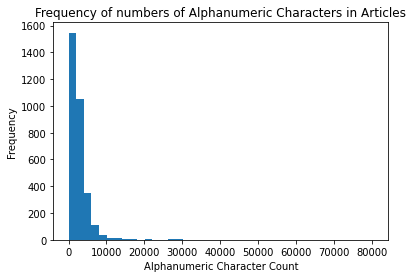
\includegraphics[scale=0.5]{hist1.png}
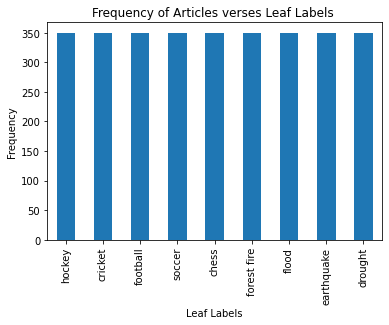
\includegraphics[scale=0.3]{hist2.png}
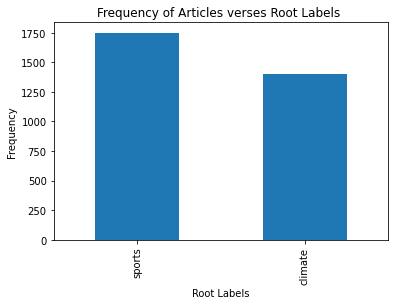
\includegraphics[scale=0.3]{hist3.png}
\newline We see that the majority of the articles are clustered between containing 0 to 4000 alphanumeric characters, with a few reaching up to 10000 words. The frequency past 10000 diminishes to a negligible amount. We see that there is an even split of articles between leaf labels, which leads to a $3:5$ split between sports and climate articles. Note that this is ideal for a multi class classification  
\section*{Binary Classification}
In the first part of our project, we worked on classifying articles into either a \texttt{"sports"} label or a \texttt{"climate"} label. This is in essence a binary classification problem as we only have two options. 
\subsection*{Problem 2}
We began by splitting our data-set randomly into training and testing data, such that a fifth of the data is used as testing data. This gave us $2520$ training samples and $630$ testing samples. 
\subsection*{Problem 3}
We begin by preprocessing our data for analysis. This involves two key steps—cleaning the data and either stemming or lemmatizing the data. For the cleaning, we used provided cleaning function, which primarily removes HTML artifacts, and added a few lines to remove underscores. \\\\
Stemming refers to a method where we remove the ends of words to shorten them to the "root". This allows us to shorten words like "run" and "running" both to "run". However, stemming often leads to results such as shortening both "stripes" and "stripping" to "strip". Still, stemming runs extremely fast, making it advantageous in the case that we don't care as much about accuracy, or in the case that our data is extremely large.
\\\\
Lemmatizing on the other hand identifies the part of speech and uses a look-up table to identify words like "stripes" to be nouns. As such, lemmatization leads to a larger dictionary size than stemming. While this method is more accurate than stemming, it runs far slower, making it not ideal in cases where minimizing runtime is important. \\\\
\\\\
Next, we apply two different methods of analyzing the preprocessed article data; these are "BOW" and "TF-IDF". "BOW" is a crude algorithm where we simply analyze the frequency of each word in a specific article relative to the entire data set to form sparse matrices for each article. "TF-IDF" considers the uniqueness of words to the document and essentially attaches a weighting factor so that the system is not overloaded with contextual data. We weight this with a logarithm as such: $$\text{TF-IDF}(d,t)=\text{TF}(t,d)\times\text{IDF}(t)$$
$$\text{IDF}(t)=\log\left({\dfrac{n}{\text{DF}(t)}}\right)+1$$
In this case, $\text{TF}(t)$ is simply the term frequency following preprocessing,  $\text{IDF}(t)$ is the inverse document frequency, $n$ is the number of articles, and $\text{DF}(t)$ is the number of documents that contain the word $t$. 
In python we are able to adjust a $min_df$ parameter, which allows us to ignore words that appear in less than minimum we can define. As we increase this parameter, the dictionary has less words in it as our tolerance for declaring words as relevant or irrelevant decreases. \\\\
Note that we will be using lemmatization for the rest of the models in this report unless otherwise stated. For lemmatization, we should remove stopwords, punctuations, and numbers after lemmatization so that the lemmatizer is able to consider the placement of words based on the sentence structure. \\\\
Completing the preprocessing, lemmatization, and then running TF-IDF, we are left with a matrix of shape $(2520, 15761)$ for training set, and $(630, 15761)$ for the testing set. The reason we have $15761$ for both is because we are fitting the TF-IDF dictionary formed from the training set onto the testing set. 

\subsection*{Problem 4}
For the next portion of the project, we dealt with dimensionality reduction. The sheer amount of data we have meanst hat many of our feature vectors are redundant or not useful. In this case, our algorithms will take an unreasonable amount of time to run. We use two main algorithms—LSI and NMF. Note from this point, we will refer to our TF-IDF processed data matrix as $\textbf{X}$\\\\
LSI refers to Latent Semantic Indexing. In this case, we begin with singular value decomposition to acquire $\textbf{X}=\textbf{U}\Sigma\textbf{V}^T$ where $\textbf{U}$ and $\textbf{V}$ are orthogonal. We then use the first $k$ columns of $\textbf{V}$ corresponding to singular values in $\Sigma$ so we have a $\textbf{V}_k$ which contains the principal components. In this case, we note that LSI is a simpler to run form of principal component analysis.  \\\\
NMF refers to Non-negative Matrix Factorization. In this case, we try to find $\textbf{W}$ and $\textbf{H}$ such that $||\textbf{X}-\textbf{WH}||^2_F$ is minimized. Note that we are using the Frobenius norm. Following this, $\textbf{W}$ acts as our dimensionality reduced data matrix. Note that $\textbf{W}$ has less rows than $\textbf{X}$, so we have less topics to describe documents with—we then fit these topics to the test documents as well. To fit this onto the test documents, we solve the optimization problem $$\text{min}_{\textbf{W}_t\geq 0}||\textbf{X}_t-\textbf{W}_t\textbf{H}||^2_F$$
Note that $\textbf{H}$ is kept consistent, so we are trying to derive a dimensionality reduced version of the test set, which will be $\textbf{W}_t$. 
\\\\
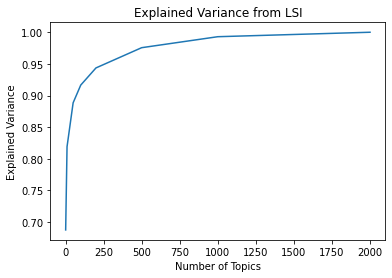
\includegraphics[scale=0.5]{explainedVariance.png}\\
Running LSI on our lemmatized data, we can set the number of features we consider as a parameter $k$. Plotting the explained variance for various values of $k$ gives us the above plot. Note that explained variance ratio refers to the amount of variance that is explained by the given $k$. As such, we see that the faster the plot plateaus (concavity), the less topics we need. \\\\
Next, we will calculate the reconstruction residual MSE for LSI and NMF—that is: \\$||\textbf{X}-\textbf{WH}||^2_F$ for NMF and $||\textbf{X}-\textbf{U}_k\Sigma_k\textbf{V}_k^T||^2_F$ for LSI. Computing these values gives us 448.072 for LSI and 451.240 for NMF. LSI has less error, although the difference seems somewhat negligible. This can be explained quite simply by observing the formulas for MSE. We note that we arrive at LSI using singular value decomposition. As such, $\textbf{U}_k\Sigma_k\textbf{V}_k^T$ must be the best approximator for $\textbf{X}$. However, NMF must randomly converge to this value, and thus must always have greater than or equal to the amount of error LSI has. 
\subsection*{Problem 5}
For this part of the project, we finally deal with the classification model. For this, we began by using a Support Vector Machine, as it is efficient as dealing with sparse matrices like the ones that we have. In essence, what we are doing is defining a hyperplane as decision boundary between the two classified classes. Thus, we are minimizing the following cost functionWe then have a trade-off parameter $\gamma$ that controls relative importance of the two components of the objective function. In this case, a softer margin, or a smaller $\gamma$ allows for a margin to classify data when it is too hard to separate by not penalizing as much in the cost function. Meanwhile, a harder margin, or a larger $\gamma$ penalizes more when a wrong classification is made. \newline
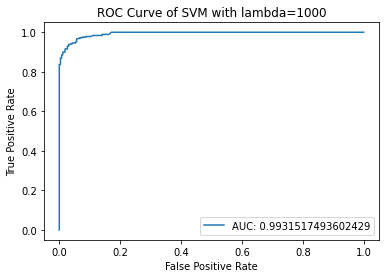
\includegraphics[scale=0.28]{roclambda1000.png}
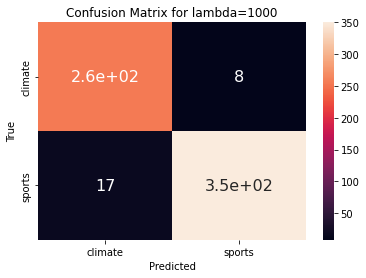
\includegraphics[scale=0.28]{conflam1000.png}
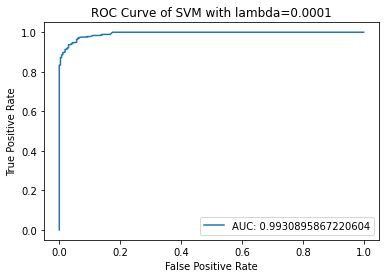
\includegraphics[scale=0.28]{lambda01roc.png}
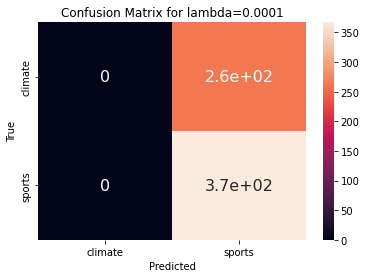
\includegraphics[scale=0.28]{comflam10.png}
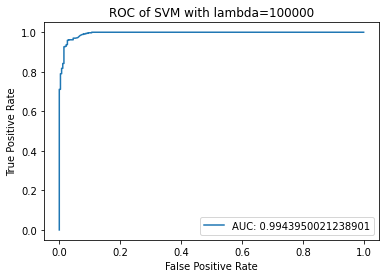
\includegraphics[scale=0.28]{highlamroc.png}
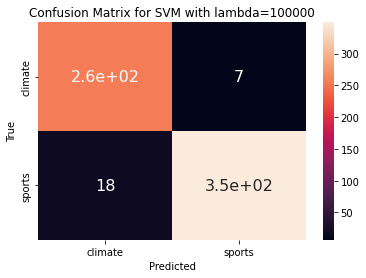
\includegraphics[scale=0.28]{highlambdacm.png}
\resizebox{0.5\textwidth}{!}{
\begin{tabular}{|c||c|c|c|c|}
\hline
\multicolumn{5}{|c|}{Comparing $\lambda$ values for SVM} \\
\hline
$\lambda$ & Accuracy & Recall & Precision & F1 Score \\
\hline
 $\lambda=1000$ & 0.960 & 0.970 & 0.938 & 0.953 \\  
 $\lambda=0.0001$ & 0.583 & 0 & 0 & 0    \\
 $\lambda=100000$ & 0.960 & 0.973 & 0.934 & 0.953 \\
 \hline
\end{tabular}
}
\\\\
We see that the ROC curves are somewhat similar in this scenario, but the climb is sharper for the hard margin. Note the confusion matrix for the soft margin SVM—there is a very low rate of classification error when it comes to the \texttt{sports} class, but a very high one when it comes to the \texttt{climate} class. This implies that due to the relaxed margin, the SVM is unable to differentiate betweeen the two classes. This happens as the number of support vectors increases,  meaning that the hyperplane we are using as our decision boundary has high variance and extremely low bias. Note that the ROC curve does not reflect this inability to classify because of the low rate of classification error when it comes to the $\texttt{sports}$ class.
\\
We see that when the value of $\lambda$ reaches extremely high values, it doesn't affect the confusion matrix at all compared to $\lambda=1000$. At this point, we can simply use the smaller regularization content.
\\\\
Next, we used 5-fold cross validation to find the best value of $\gamma$, using average validation accuracy as the scoring metric. This involved an exhaustive search, using grid search, where we compare accuracy across $10^k|-3\leq\lambda\leq 5$. Note we used integer powers of $10$. This gave us the best parameter of $100000$, which we used from this point on. Note the accuracy, precision, and F1 score are given in the above table. 


\subsection*{Problem 6}
After the SVM, we use a different model—this time we use a logistic regression. We use a logistic function $h$ and apply it to the feature vectors to find optimal weights. 
$$h(\textbf{X})=\dfrac{1}{1+e^{-\theta^T\textbf{X}}},\theta=f(\textbf{W},b)$$
We then minimize cross entropy loss and in the process add a regularization term to it, which we express as $\frac{1}{C}R(f)$. As such, there are two types of regularization we will be using for $R(f)$ which are L1 and L2 regularization, while we can adjust $C$ as our hyperparameter. \\\\
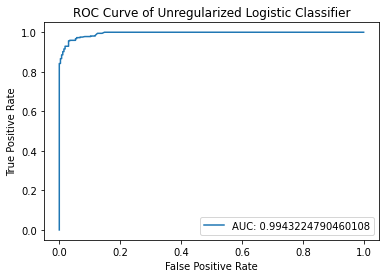
\includegraphics[scale=0.3]{unreglogroc.png}
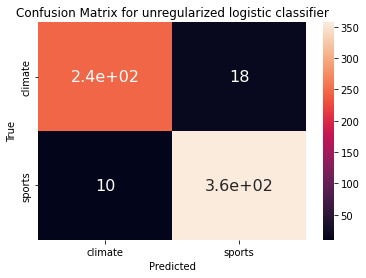
\includegraphics[scale=0.3]{unreglogcm.png}

Next, we tune the regularization strength, by taking $k$ such that $10^k|-3\leq C\leq 5$ and then conducting an exhaustive search similar to before. Using 5-fold cross validation and scoring based on accuracy, we find that our optimal parameter for $L1$ is $C=10$, and for $L2$ is $C=500$. From this point, for $L1$ and $L2$ regularized logistic models, we assume that we are using these optimal parameters. \\

\resizebox{0.45\textwidth}{!}{
\begin{tabular}{|c||c|c|c|c|}
\hline
\multicolumn{5}{|c|}{Comparing logistic classification regularization models} \\
\hline
Regularization & Accuracy & Recall & Precision & F1 Score \\
\hline
None & 0.956 & 0.932 & 0.961 & 0.946 \\  
L1 & 0.962 & 0.973 & 0.938 &  0.955    \\
L2 & 0.962 & 0.970 & 0.941 & 0.955   \\
 \hline
\end{tabular}
}
\\\\
Using these optimal parameters, we are able to compare Accuracy, Recall, Precision, and F1 Scores across the unregularized, L1 regularized, and L2 regularized logistic models. We see that the unregularized model performed the worst in terms of accuracy, while the L1 and L2 performed about the same to the point where they had the same F1 Score. Note that the differences between L1 and L2 seem almost negligible. \\\\
Regularization should make our model better at generalizing its results to test results by increasing bias. As such, as our regularization constant $C$ increases, we are regularizing less and as such our models should be more accurate, while our learnt coefficients should be smaller. We see this reflected in the fact that recall is far better without regularization. However, in this specific case, we see that the regularization helped to generalize to the test data, so we did not reach a regularization constant where our models became inaccurate, but rather simplified our model to generalize better. 
\\\\
Note that L1 regularization simplifies by minimizing the sum of the magnitudes of the weights, while L2 simplifies by minimizing the sum of the squares of the weights. This means that L1 regularization is more likely to simply zero-out some of the weights, meaning that we will likely have a sparse matrix. meanwhile, for L2, we will be left with very small values instead of zeroes. This means that L1 regularization is better at dealing with data very far from the decision boundary. We will be using L1 regularization, as computation with sparse matrices is also less expensive in this case. 
\\\\
Comparing the logistic regression and linear SVM, we see that both are using a linear decision boundary. However, logistic regression relies on a more probabilistic approach—that is, it gives us a set of probabilities based on its confidence. SVM on the other hand simply constructs a hyperplane as a decision boundary between two classified classes that maximizes the margin between the two classes. This maximum in our case is determined by the Frobenius norm. This leads us to the conclusion that the SVM is more geometric in nature while the logistic regression is more probabilistic in nature. \\\\
This difference is not statistically significant here, as the accuracy is about the same for both. Note also that SVM is simpler, so it generalizes better than the logistic regression model, although we can adjust the regularization constant. This also means that SVM will generally run faster than logistic classification, so for large data, SVM is preferred. However, in cases where the distance from the margin made by the hyperplane boundary is very large for some entry, logistic regression will be better at classifying this said data. This makes sense due to the probabilistic nature of the logistic classification model. 
\subsection*{Problem 7}
The final classifier we tested is the Gaussian Naive Bayes classifier. We assume the data given takes the form of a Gaussian distribution. This classifier calculates labels by minimizing the probability of wrongly classifying some entry. This is extremely simple and relies on an extended version of Bayes' theorem: $$Y_{\text{pred}}=\text{argmax}_{r\in{1,...,r}} P(Y=r)\prod_{i=1}^n P_r(x)$$
In this case, we are simply taking the most likely label. Note that it is naive as we are assuming all of our features are mutually independent. \\\\
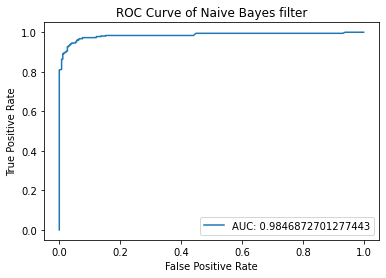
\includegraphics[scale=0.3]{naivebaesroc.png}
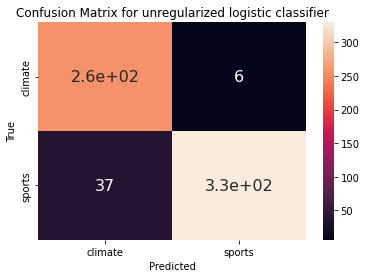
\includegraphics[scale=0.3]{ypredgauss.png}
\resizebox{0.45\textwidth}{!}{
\begin{tabular}{|c|c|c|c|}
\hline
\multicolumn{4}{|c|}{Scoring Metrics for Naive Bayes classifier} \\
\hline
Accuracy & Recall & Precision & F1 Score \\
\hline
 0.932 & 0.977 & 0.874 & 0.923 \\  
 \hline
\end{tabular}
} \\\\

We see that our accuracy, unsurprisingly for such a simplistic model, does not perform as well as the SVM or the logistic classifier. 

\subsection*{Problem 8}
Our final task for binary classification is grid search. For grid search, we take a list of hyper parameters and perform an exhaustive search to try to determine the most accurate combination. We thus construct a pipeline of the following steps:\\
\textbf{Module 1.} Clean the data \\
\textbf{Module 2.} Lemmatize or Stem the data \\
\textbf{Module 3.} Change minimum document frequency for TF-IDF between 3 and 5 \\
\textbf{Module 4.} Choose dimensionality reduction model (LSI or NMF) with parameters
\textbf{Module 4.} Choosing between SVM, Logistic Regression with L1 or L2 regularization, and Naive Bayes Model
\\\\
Combinatorically trying all possible combinations, we came up with the five best combinations listed below:\\
\textbf{1.} Cleaned, Lemmatized, Logistic Regression with L1 regularization, LSI with 80 components, $\text{min\_df}$ of 5 \\
\textbf{2.} Cleaned, Stemmed, Logistic Regression with L2 regularization, LSI with 80 components, $\text{min\_df}$ of 5\\
\textbf{3.} Cleaned, Stemmed, Logistic Regression with L1 regularization, LSI with 80 components, $\text{min\_df}$ of 5\\
\textbf{4.} Dirty, Lemmatized, Logistic Regression with L2 regularization, LSI with 80 components, $\text{min\_df}$ of 5 \\
\textbf{5.} Dirty, Lemmatized, Logistic Regression with L1 regularization, LSI with 80 components, $\text{min\_df}$ of 5 \\\\
First, note that the above are not ranked but rather simply listed. We notice that within the top 5, all use logistic regressions, LSI with 80 components, and a minimum document frequency for TF-IDF of 5. We also note that the regularization parameter does not seem to matter too much, which aligns with our findings earlier where they had the same F1 Score.  Next, we applied the models to the testing set. \\\\

\resizebox{0.45\textwidth}{!}{
\begin{tabular}{|c|c|c|c|c|}
\hline
\multicolumn{5}{||c||}{Accuracy of Grid-searched Models} \\
\hline\hline
Model No. & Accuracy & Recall & Precision & F1 Score\\
\hline
1 & 0.968 & 0.981 & 0.945 & 0.963\\
2 & 0.966 & 0.981 & 0.941 & 0.961\\
3 & 0.968 & 0.981 & 0.945 & 0.963\\
4 & 0.965 & 0.977 & 0.941 & 0.959\\
5 & 0.965 & 0.977 & 0.941 & 0.959\\
 \hline
\end{tabular}
} \\\\
Note that the Model No. are defined previously and are once again not a ranking. We see that cleaning seems to improve the models, but there isn't much of a difference between stemming and lemmatizing. This suggests that stemming would be the better option as it is less complex;however, lemmatization ran faster on our machines. We attributed this to the caching system coded into our Gridsearch.
\section*{Multi-class classification}
\subsection*{Problem 9}
The next problem we address in our project is multi-class classification—that is, given the articles, we identify the respective $\texttt{leaf\_label}$. Towards this goal, we apply two primary models. First, we have the Naive Bayesian classifier, whose application here is analogous to its application in binary classification. Next, we have multiclass SVM classification. \\\\ %insert explanation of multiclass SVM models
In order to use SVM for multiclass classification, there are two popular methods. One versus One (OvO) trains cC2 classifiers, covering every possible combination of classes. The predicted class is then selected with a majority vote. One versus Rest (OvR) trains C classifiers, each performing binary classification between a class of interest and the union of all the rest of the classes.\\\\
Since the collection of other classes in one vs rest is far more numerous than the class of interest, it could bias our SVM. We counteracted the imbalance by weighing the class of interest and all other classes  inversely proportional to their respective counts. This was done for every class and the decisions scores for each was used to vote on the final prediction, with the highest score winning. \\\\
\resizebox{0.45\textwidth}{!}{
\begin{tabular}{|c||c|c|c|c|}
\hline
\multicolumn{5}{|c|}{Scoring Metrics for Multiclass Classifiers} \\
\hline
Model & Accuracy & Recall & Precision & F1 Score \\
\hline
Naive Bayes & 0.751 & 0.741 & 0.734 & 0.732 \\  
One vs One & 0.790 & 0.782 & 0.787 &  0.782    \\
One vs Rest & 0.904 & 0.900 & 0.902 & 0.898   \\
 \hline
\end{tabular}
} \\\\
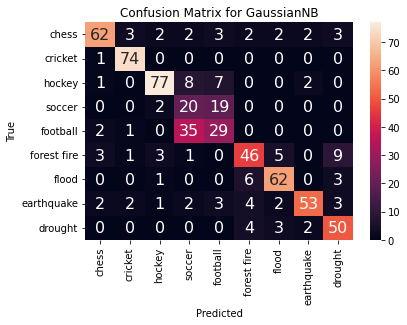
\includegraphics[scale=0.5]{multGaussNB.png} \\
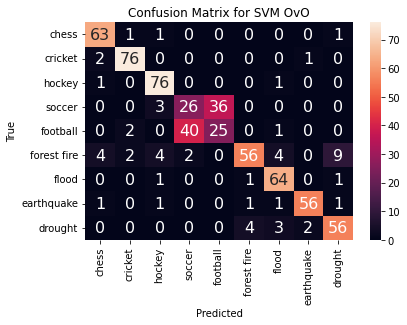
\includegraphics[scale=0.5]{multSVMOVO.png}
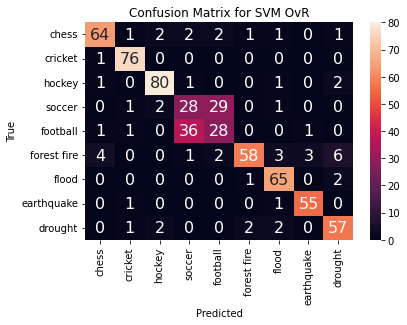
\includegraphics[scale=0.5]{multSVMOVR.png} \\\\
It is clear simply by observing the scoring metrics that the OvR SVM classification method worked the best. However, we note that although generally the confusion matrices are more dense around the diagonal, as it should be, there is a distinct block around \texttt{"football"} and \texttt{"soccer"} in all three of our models. This makes sense, as the model is likely conflating articles in which the term "football" is present; it could refer to either American football or soccer in countries outside the United States. As such, we considered moving soccer and football into one combined label to increase accuracy. \\\\
Class imbalance could bias our SVM to make it more inclined to predict the most popular class. Similarly to how we implemented OvR, the class imbalance caused by the merging of labels was solved by weighing the classes.\\\\
\resizebox{0.45\textwidth}{!}{
\begin{tabular}{|c||c|c|c|c|}
\hline
\multicolumn{5}{|c|}{Scoring Metrics for Merged Multiclass Classifiers} \\
\hline
Model & Accuracy & Recall & Precision & F1 Score \\
\hline 
One vs One & 0.905 & 0.900 & 0.902 &  0.898    \\
One vs Rest & 0.919 & 0.915 & 0.915 & 0.913   \\
 \hline
\end{tabular}
} \\
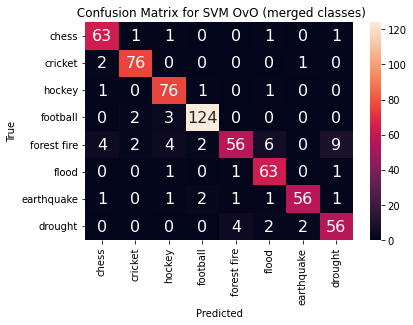
\includegraphics[scale=0.5]{multiOVOMERGE.png}
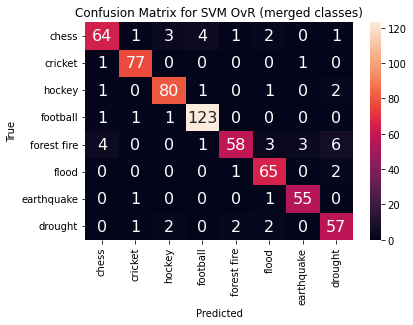
\includegraphics[scale=0.5]{multiOVRMERGE.png}\\\\
We see that the accuracy of our model for the merged labels is far higher than the prior accuracy. This is also observed in the confusion matrix where we have an extremely dense diagonal, with only a few misclassifications.

%class imbalance
\section*{Word Embedding}
\subsection*{Problem 10}
\textit{(a)} By comparing the co-occurrence probabilities, we can distinguish between words that are words that are relevant and words that are irrelavant.\\\\
\textit{(b)} This will depend on the circumstances, if we are inferencing a pretrained GLoVE implementation to convert each word in the sentence to vectors, then yes it will return the same vector. This is because GLoVE acts like a dictionary when being inferenced and thus doesn't take into account context.\\\\
On the other hand if we are training GLoVE on data that includeds the sentence “James is running in the park.” and other sentences, and we swap it out for "James is running for the
presidency." Then yes, the resulting embedding for "running" would be different since the co-occurrence probabilities would now be different.\\\\
Furthermore, if we only train GLoVE on this sentence “James is running in the park.” with "James is running for the
presidency." Then the embedding wouldn't change, since we are swapping out words that occur once, with words that previously weren't part of the sentence, and GLoVE doesn't take into consideration what each word is, only
the co-occurence probabilities.\\\\
\textit{(c)} For two vectors $a$ and $b$, we have that
$$||a-b||^2=||a||^2+||b||^2-2a\cdot b$$
In our case we have that $a=$GLoVE["queen"] - GLoVE["king"] and $b=$GLoVE["wife"] - GLoVE["husband"]. Therefore we can view this as a word analogy problem. It makes sense that husband is the expected answer to the question "a queen is to a king as a wife is to a \_?" for the "\_?". Therefore we would expect the angle between $a$ and $b$ to be 0, as a result we have
$$||a-b||^2=(||a||-||b||)^2$$
As a result we would expect:
$$||a-b||=||a||-||b||$$
Where $a=$GLoVE["queen"] - GLoVE["king"] and $b=$GLoVE["wife"] - GLoVE["husband"].\\\\
\textit{(d)}
We would rather lemmatize than stem, because lemmatize takes into the contex surounding the word, and attempts to preserve the meaning of the word. In contrast there is no guarantee that stemming will preserve the meaning of the word.
% \begin{enumerate}
% \item[(a)] 
% Because then it can distinguish between relevant words and irrelevant words.
% \item[(b)]
% It will be different since the context is now different.
% \item[(c)]
% From the triangle inequality we would expect:
% \begin{multline*}
%     ||\text{GLoVE["queen"] - GLoVE["king"] - GLoVE["wife"] + GLoVE["husband"]}||_2\leq\\
%     ||\text{GLoVE["queen"] - GLoVE["king"]}||_2+||\text{GLoVE["wife"] -GLoVE["husband"]}||
% \end{multline*}
% \item[(d)]
% I would rather lemmatize, because that would take into the context of the 
% word when lemmatizing it unlike stemming.
% \end{enumerate}
\subsection*{Problem 11}
\textit{(a)} We used the following feature engineering process: To generate 
the features for article $i$, we first converted all of the  \texttt{"full\_text"}, \texttt{"summary"}, and \texttt{"keywords"} words into GLoVE embeddings. For future convenience let us denote these three, \texttt{"full\_text"}, \texttt{"summary"}, and \texttt{"keywords"}, as the "data sources" for a article\\\\
To convert each word, we first cleaned it, ie we converted it to lower case and removed all non alphabet letters. Let us denote $w_{ijk}$ be the GLoVE emebedding for the $k$th word, from the $i$th article, and from the $j$th data source, ie $j=0$ if the word comes from 
the \texttt{"full\_text"} of the article, $j=1$ if the word comes from the \texttt{"summary"} of the article, and $j=2$ if the word comes from the \texttt{"keywords"} of the article. If a word did not occur in the glove embedding, we simply had $w_{ijk}=\textbf{0}$. To aggregate these embeddings we first took the average for each of these, ie we have 
$$X_{ij}=\frac{1}{n_{ij}}\sum_{k=1}^{n_{ij}} w_{ijk}$$
Where $n_{ij}$ is the number of words in the $j$th data source from the $i$th article. However we must aggregate the three $X_{i0},X_{i1},X_{i2}$ vectors into one vector which we can train our model on. And because of the requirement that the inputs from the model must be of the same dimension
as the GLoVE emebddings, we decided to aggregate the three in the following way:
$$X_i=C_0 X_{i0}+ C_1 X_{i1}+C_2 X_{i2}$$
For some weighting hyperparmaeters $C_0$, $C_1$, $C_2$. We discuss how we selected them in the following section.\\\\
\textit{(b)}
We trained a SVM with a linear kernel on the dataset with the feature engineering process we described above. We trained the SVM in the following method, we held out 20\% of the data as a test set, and then for the other 80\% we conducted trained 5 models on it through 5 fold cross validation. We this train-validation-test split because it allowed us to not only optimize the model but also the hyperparameters $C_0$, $C_1$, $C_2$.\\\\
The first method we attempted to use to optimize inspired by gradient descent. We would want to optimize the accuracy which we can view as a function $f$ of the hyperparameters $C_0$, $C_1$, $C_2$. If $f$ was a differentiable function we would have that the gradient descent algorithm could be written as:
$$C_i\leftarrow C_i+\lambda \frac{\partial f}{\partial C_i}$$
However we do not know what is the expression for $f$ in terms of $C_i$,
and thus we do not know the term for the derivative either. Therefore we tried an approach were we estimated the partial derivative of $f$ with respect to $C_0$ (and in a similar fashion the partial derivative with respect to $C_1$ and $C_2$).
\begin{multline*}
    \frac{\partial f(C_0,C_1,C_2)}{\partial C_0}\approx \frac{1}{\Delta C}
    (f(C_0+\Delta C,C_1,C_2)-\\ f(C_0,C_1,C_2))
\end{multline*}
However experimentation with this method finds that $f$ is a highly non convex function. And as a result gradient descent is very susceptible to the starting position and very vurnerable to fall into local maximums.\\\\
Therefore the next method we tried was simple grid search, but we found that the number of permutations we would have to iterate over made it such that finding the optimal permutation of $C_0$, $C_1$, $C_2$ to more than 1 digit of accuracy to take too long.\\\\
As a result we implemented a variation on bisection search to find the optimal $C_0$,$C_1$,$C_2$. Our algorithm was as follows:\\\\
\textbf{Algorithm 1} \textit{For a space bound by $C_0\in (C_{0_{min}},C_{0_{max}})$, $C_1\in (C_{1_{min}},C_{1_{max}})$, and $C_2\in (C_{2_{min}},C_{2_{max}})$, do the following:}\\\\
\textbf{Step 1.} \textit{Divide up $C_0\in (C_{0_{min}},C_{0_{max}})$ in half to form a set of two sets of possible values of $C_0$, ie form a set: $\left(C_0\in (C_{0_{min}},\frac{C_{0_{min}}+C_{0_{max}}}{2}), 
C_0\in (\frac{C_{0_{min}}+C_{0_{max}}}{2},C_{2_{max}})\right)$
and doing likewise for $C_1$ and $C_2$. Then taking the Cartesian product
between these 3 sets to form 8 subspaces.
}
\\\\
\textbf{Step 2.} \textit{For each subspace, calculate the accuracy with $C_0$, $C_1$, $C_2$ being the center of this subspace}\\\\
\textbf{Step 3.} \textit{Recursively call this function on the subspace that produces the best accuracy as calculated in Step 2.}\\\\
Starting off from the space of $C_0,C_1,C_2\in (-1,1)$ we are able to find $C_0,C_1,C_2$ such that the accuracy on the test set was $96.82\%$, with an
optimal $C_1=-0.560546875$, $C_2=-0.904296875$, $C_3=-0.677734375$. See figure below for the corresponding confusion matrix of this classifier we trained with hyperparamaters tuned using this method.\\\\
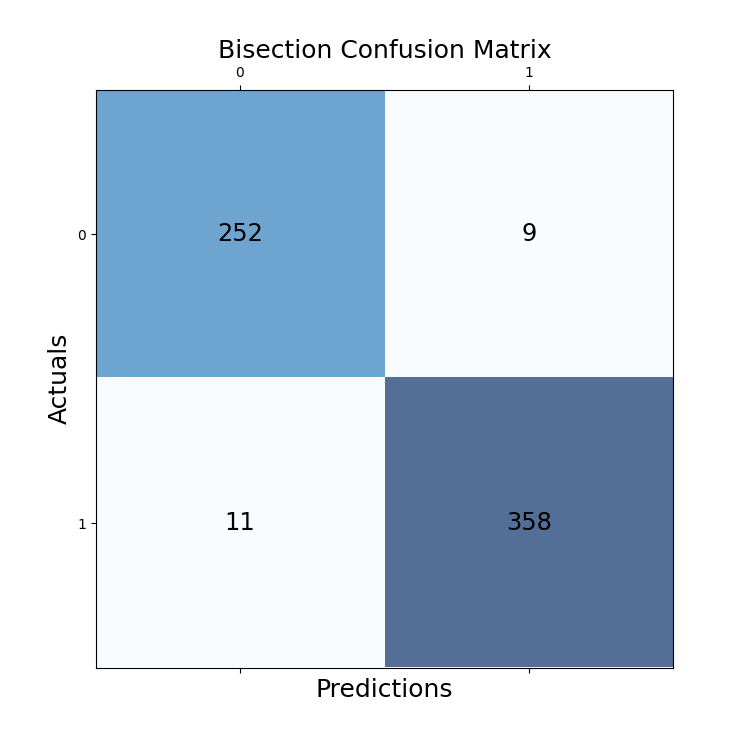
\includegraphics[scale=.4]{bisection_confusion_matrix.png}
However this method has a weakness in that it needs the accuracy, or $f$
to be symmetric around the maximum. Therefore we also experimented with the 
optimization method proposed by Carrillo et al in \textit{A consensus-based global optimization method for high
dimensional machine learning problems
}. This method can be roughly characterized as a optimization method using particles that are influnced through component wise brownian motion, and which the authors claim is more effective than gradient descent for non convex functions.\\\\
We used 10 particles, and with $\lambda=0.3$, $\gamma_{k,\theta}=1$, $\sigma_{k,\theta}=0.1$, $\beta=0.9$, and trained them for 50 epochs without minibatching. The model converged as can be seen from the figures below. \\
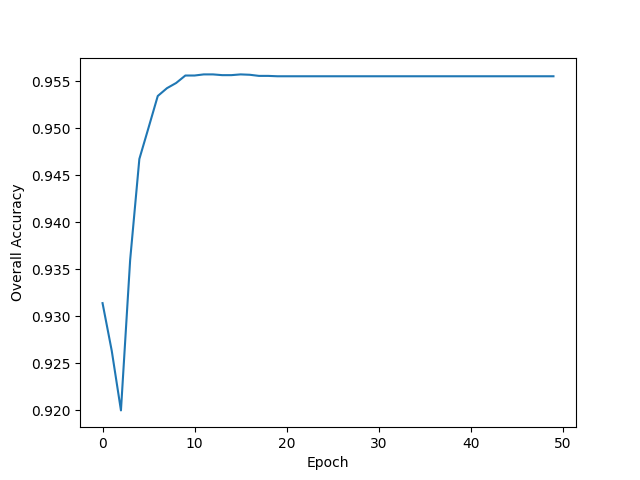
\includegraphics[scale=0.25]{overall_accuracy.png}
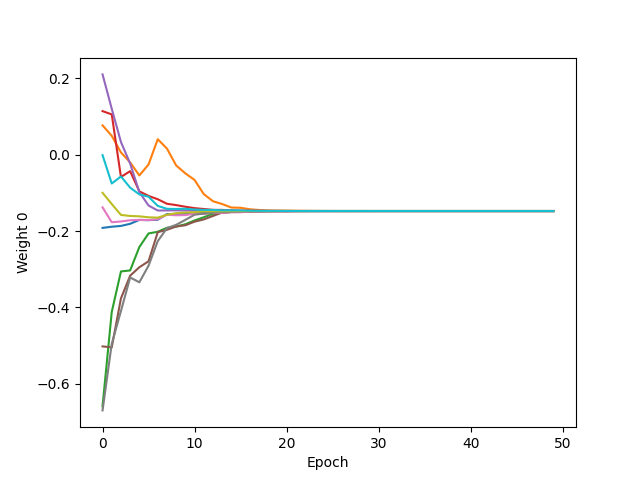
\includegraphics[scale=0.25]{weight_0.png}\\
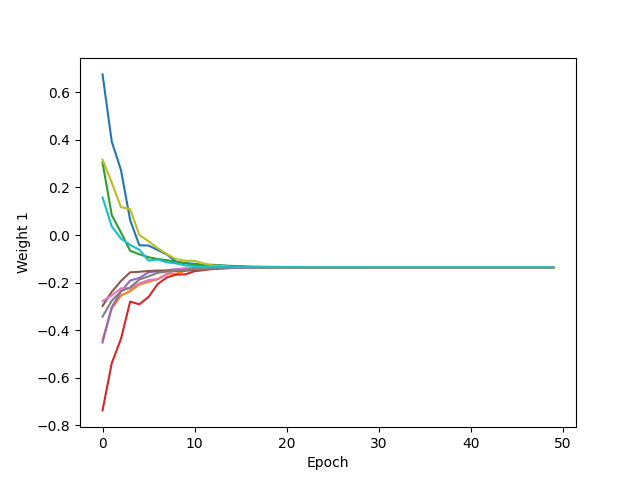
\includegraphics[scale=0.25]{weight_1.png}
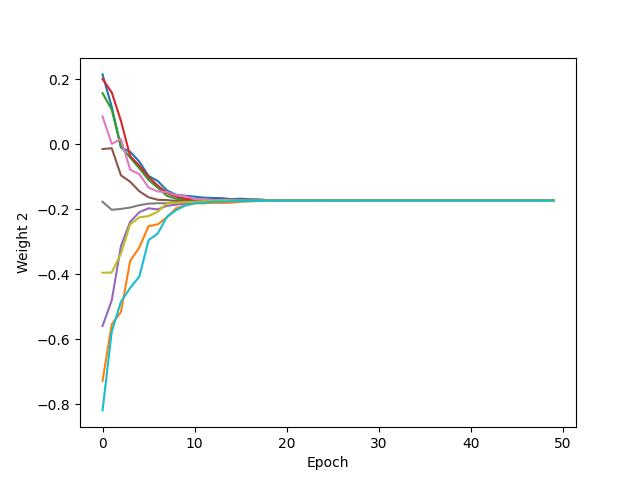
\includegraphics[scale=0.25]{weight_2.png}
The first figures shows the average accuracy, and the next 3 plot shows the 
$C_1$, $C_2$, and $C_3$ for each particle and how they all converge. This optimizer results in finding the following optimal values for $C_0,C_1,C_2$,
we get  $C_0=-0.14766396$ and $C_1=-0.13540619$ and $C_2=-0.1732398$, and as a result an accuracy of $96.19\%$ on the test set. The confusion matrix is shown below\\
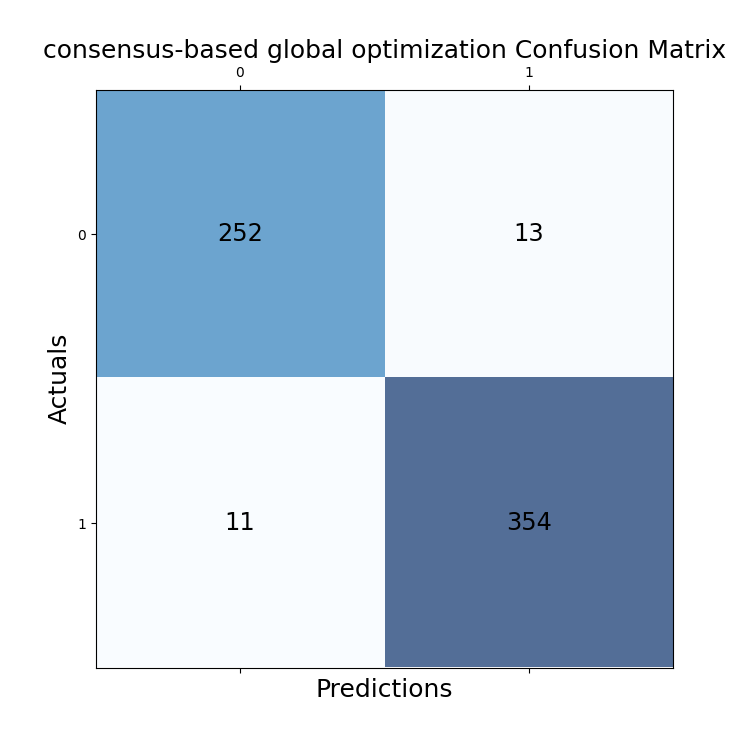
\includegraphics[scale=.4]{stochastic_confusion_matrix.png}\\
Therefore since the bisection method shows slightly better performance and is significantly faster than the consensus-based global optimization method, we will use it to for the next two problems.
\subsection*{Problem 12}
Using the train test validation split and bisection search methods described in Problem 11, we get the following plot for the accuracy vs the dimensions of the GLoVE Embedding:\\
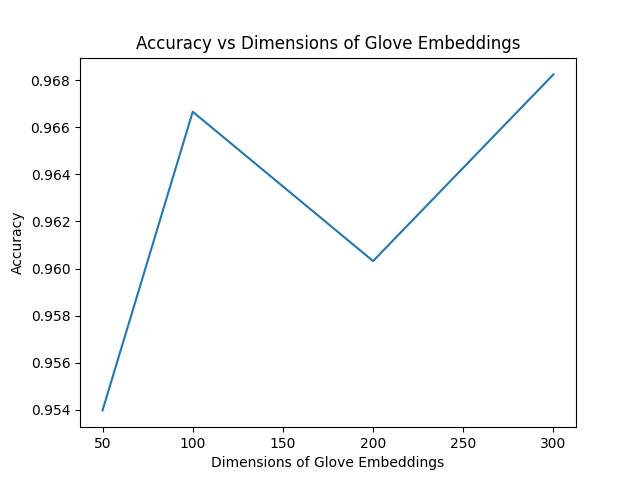
\includegraphics[scale=0.45]{Problem11.png}\\
The trend observed seems to be that increasing the dimensions does increase the accuracy overall, except for when the GLoVE dimensions is 200, in which case the accuracy is actually lower than the cases with GLoVE dimension of 100. Beyond this dip when the GLoVE dimensions is 200, this is expected, because more dimensions will allow the model to have more parameters to optimize over, up until the point where there becomes too many parameters availble to optimize over and the model beings to overfit.
\subsection*{Problem 13}
Once again, using the train test validation split and bisection search methods described in Problem 11, we get the following visulaizations with UMAP:\\
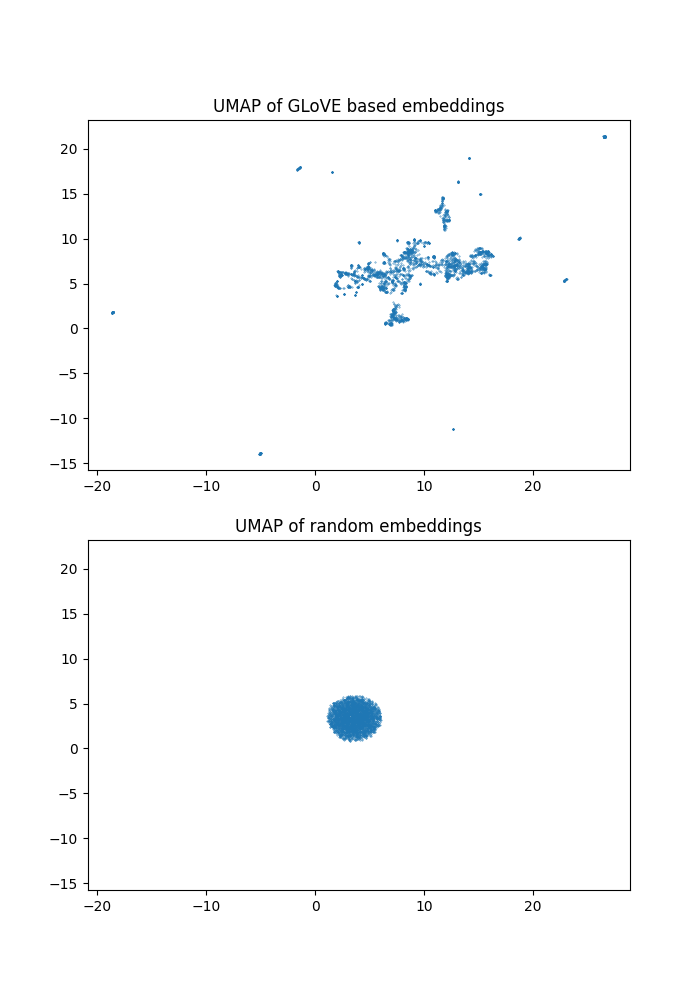
\includegraphics[scale=0.4]{UMAP_unlabeled.png}\\
As we can see, the UMAP visualization for the GLoVE based embedding form multiple clusters. In comparison the random embeddings is just visualized as one "ball". We investigate further by including the labels for each plot below.\\
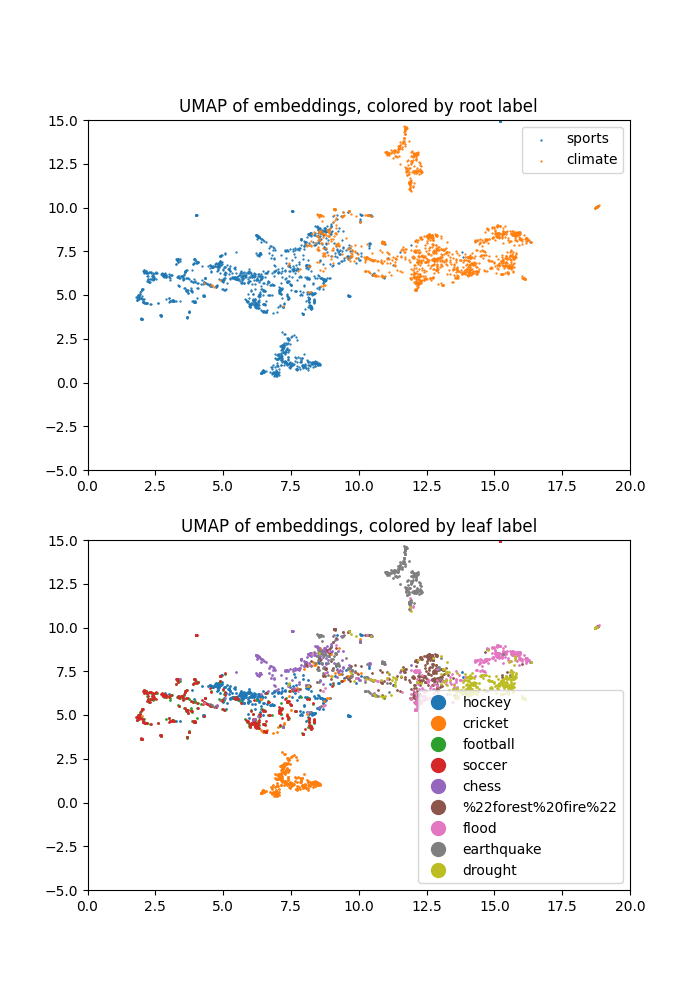
\includegraphics[scale=0.4]{UMAP_labeled.png}\\
As can be seen we set the y and x limits of the plot to (0,20) and (-5,15)
respectively to remove the outliers and allowing us to observer more detail in the "Central cluster". From the plots, we can draw some interesting observations, for instance the sports that are less "physcial" such as chess, is visualized as more closely to climate articles.
\end{multicols}
\end{document}